%%%%%%%%%%%%%%%%%%%%%%%%%%%%%%%%%%%%%%%%%%%%%%%%%%%%%%%%%%%%%%%%%%%%%%%%%%%%%%%%
%% Plantilla de memoria en LaTeX para la ETSIT - Universidad Rey Juan Carlos
%%
%% Por Gregorio Robles <grex arroba gsyc.urjc.es>
%%     Grupo de Sistemas y Comunicaciones
%%     Escuela Técnica Superior de Ingenieros de Telecomunicación
%%     Universidad Rey Juan Carlos
%% (muchas ideas tomadas de Internet, colegas del GSyC, antiguos alumnos...
%%  etc. Muchas gracias a todos)
%%
%% La última versión de esta plantilla está siempre disponible en:
%%     https://github.com/gregoriorobles/plantilla-memoria
%%
%% Para obtener PDF, ejecuta en la shell:
%%   make
%% (las imágenes deben ir en PNG o JPG)

%%%%%%%%%%%%%%%%%%%%%%%%%%%%%%%%%%%%%%%%%%%%%%%%%%%%%%%%%%%%%%%%%%%%%%%%%%%%%%%%

\documentclass[a4paper, 12pt, english]{book}
\usepackage[T1]{fontenc}


\usepackage[a4paper, left=2.5cm, right=2.5cm, top=3cm, bottom=3cm]{geometry}
\usepackage{times}
%\usepackage[spanish]{babel} % Comenta esta línea si tu memoria es en inglés
\usepackage{url}
%\usepackage[dvipdfm]{graphicx}
\usepackage{graphicx}
\usepackage{float}  %% H para posicionar figuras
\usepackage[nottoc, notlot, notlof, notindex]{tocbibind} %% Opciones de índice
\usepackage{latexsym}  %% Logo LaTeX

\usepackage[T1]{fontenc}
\usepackage{selinput}
\SelectInputMappings{%
  aacute={á},
  ntilde={ñ},
  Euro={€}
}
\usepackage{babel}

\usepackage{hyperref}

\usepackage{listings}
\usepackage{color}
\definecolor{nd}{RGB}{98, 143, 217}
\definecolor{keyword}{RGB}{255,51,102}
\definecolor{bg}{RGB}{255, 255, 232}
\definecolor{comment}{RGB}{73, 79, 92}
\definecolor{str}{RGB}{30, 184, 135}

\lstdefinelanguage{Sass}{
	keywords={mixin, keyframe, include, import, extend, class, \@},
	keywordstyle=\color{keyword},
	indentifierstyle=\color{black}\bfseries,
	sensitive=false,
	comment=[l]{\#},
  	morecomment=[s]{/*}{*/},
    	commentstyle=\color{comment}\ttfamily
}

\lstdefinelanguage{JavaScript}{
 	keywords={constructor, typeof, new, true, false, catch, function, return, null, catch, switch, var, if, in, while, do, else, case, break},
  	keywordstyle=\color{keyword},
  	ndkeywords={public, Router, class, export, boolean, throw, implements, import, this,prototype, then},
  	ndkeywordstyle=\color{nd}\bfseries,
  	identifierstyle=\color{black},
  	sensitive=false,
  	comment=[l]{//},
  	morecomment=[s]{/*}{*/},
  	commentstyle=\color{comment}\ttfamily,
  	stringstyle=\color{str}\ttfamily,
  	morestring=[b]',
  	morestring=[b]"
}

\lstset{
frame=single,
   language=Javascript,
   backgroundcolor=\color{bg},
   extendedchars=true,
   basicstyle=\small\ttfamily,
   showstringspaces=false,
   showspaces=false,
   numbers=left,
   numberstyle=\footnotesize,
   numbersep=9pt,
   tabsize=2,
   breaklines=true,
   showtabs=false,
   captionpos=b,
   xleftmargin=\parindent,
}

\title{Memoria del Proyecto}
\author{Ismael Slimane Zubillaga}

\renewcommand{\baselinestretch}{1.5}  %% Interlineado

\begin{document}

\renewcommand{\refname}{Bibliografía}  %% Renombrando
\renewcommand{\appendixname}{Apéndice}

%%%%%%%%%%%%%%%%%%%%%%%%%%%%%%%%%%%%%%%%%%%%%%%%%%%%%%%%%%%%%%%%%%%%%%%%%%%%%%%%
% PORTADA

\begin{titlepage}
\begin{center}
\begin{tabular}[c]{c c}
%\includegraphics[bb=0 0 194 352, scale=0.25]{logo} &

\includegraphics[scale=0.25]{img/logo_vect.png} &
\begin{tabular}[b]{l}
\Huge
\textsf{UNIVERSIDAD} \\
\Huge
\textsf{REY JUAN CARLOS} \\
\end{tabular}
\\
\end{tabular}

\vspace{3cm}

\Large
INGENIERÍA EN TECNOLOGÍAS DE LA TELECOMUNICACIÓN

\vspace{0.4cm}

\large
Curso Académico 2017/2018

\vspace{0.8cm}

Trabajo Fin de Grado/Máster

\vspace{2.5cm}

\LARGE
ANGULAR - ELASTICSEARCH - DASHBOARD INTERFACE

\vspace{4cm}

\large
Autor : Ismael Slimane Zubillaga \\
Tutor : Dr. Jesús M. González-Barahona
\end{center}
\end{titlepage}

\newpage
\mbox{}
\thispagestyle{empty} % para que no se numere esta pagina


%%%%%%%%%%%%%%%%%%%%%%%%%%%%%%%%%%%%%%%%%%%%%%%%%%%%%%%%%%%%%%%%%%%%%%%%%%%%%%%%
%%%% Para firmar
\clearpage
\pagenumbering{gobble}
\chapter*{}

\vspace{-4cm}
\begin{center}
\LARGE
\textbf{Trabajo Fin de Grado/Máster}

\vspace{1cm}
\large
Título del Trabajo con Letras Capitales para Sustantivos y Adjetivos

\vspace{1cm}
\large
\textbf{Autor :} Nombre del Alumno/a \\
\textbf{Tutor :} Dr. Gregorio Robles Martínez

\end{center}

\vspace{1cm}
La defensa del presente Proyecto Fin de Carrera se realizó el día \qquad$\;\,$ de \qquad\qquad\qquad\qquad \newline de 20XX, siendo calificada por el siguiente tribunal:


\vspace{0.5cm}
\textbf{Presidente:}

\vspace{1.2cm}
\textbf{Secretario:}

\vspace{1.2cm}
\textbf{Vocal:}


\vspace{1.2cm}
y habiendo obtenido la siguiente calificación:

\vspace{1cm}
\textbf{Calificación:}


\vspace{1cm}
\begin{flushright}
Fuenlabrada, a \qquad$\;\,$ de \qquad\qquad\qquad\qquad de 20XX
\end{flushright}

%%%%%%%%%%%%%%%%%%%%%%%%%%%%%%%%%%%%%%%%%%%%%%%%%%%%%%%%%%%%%%%%%%%%%%%%%%%%%%%%
%%%% Dedicatoria

\chapter*{}
\pagenumbering{Roman} % para comenzar la numeracion de paginas en numeros romanos
\begin{flushright}
\textit{Dedicado a \\
mi familia / mi abuelo / mi abuela}
\end{flushright}

%%%%%%%%%%%%%%%%%%%%%%%%%%%%%%%%%%%%%%%%%%%%%%%%%%%%%%%%%%%%%%%%%%%%%%%%%%%%%%%%
%%%% Agradecimientos

\chapter*{Agradecimientos}
%\addcontentsline{toc}{chapter}{Agradecimientos} % si queremos que aparezca en el índice
\markboth{AGRADECIMIENTOS}{AGRADECIMIENTOS} % encabezado

%Aquí vienen los agradecimientos\ldots Aunque está bien acordarse de la pareja, no hay que olvidarse de dar las gracias a tu madre, que aunque a veces no lo parezca disfrutará tanto de tus logros como tú\ldots
%Además, la pareja quizás no sea para siempre, pero tu madre sí.

%%%%%%%%%%%%%%%%%%%%%%%%%%%%%%%%%%%%%%%%%%%%%%%%%%%%%%%%%%%%%%%%%%%%%%%%%%%%%%%%
%%%% Resumen

\chapter*{Resumen}
%\addcontentsline{toc}{chapter}{Resumen} % si queremos que aparezca en el índice
\markboth{RESUMEN}{RESUMEN} % encabezado

%Aquí viene un resumen del proyecto. Ha de constar de tres o cuatro párrafos, donde se presente de manera clara y concisa de qué va el proyecto.
%Han de quedar respondidas las siguientes preguntas:

%\begin{itemize}
%  \item ¿De qué va este proyecto? ¿Cuál es su objetivo principal?
%  \item ¿Cómo se ha realizado? ¿Qué tecnologías están involucradas?
%  \item ¿En qué contexto se ha realizado el proyecto? ¿Es un proyecto
%dentro de un marco general?
%\end{itemize}

%Lo mejor es escribir el resumen al final.

%%%%%%%%%%%%%%%%%%%%%%%%%%%%%%%%%%%%%%%%%%%%%%%%%%%%%%%%%%%%%%%%%%%%%%%%%%%%%%%%
%%%% Resumen en inglés

\chapter*{Summary}
%\addcontentsline{toc}{chapter}{Summary} % si queremos que aparezca en el índice
\markboth{SUMMARY}{SUMMARY} % encabezado

%Here comes a translation of the ``Resumen'' into English. Please, double check it for correct grammar and spelling.
%As it is the translation of the ``Resumen'', which is supposed to be written at the end, this as well should be filled out
%just before submitting.


%%%%%%%%%%%%%%%%%%%%%%%%%%%%%%%%%%%%%%%%%%%%%%%%%%%%%%%%%%%%%%%%%%%%%%%%%%%%%%%%
%%%%%%%%%%%%%%%%%%%%%%%%%%%%%%%%%%%%%%%%%%%%%%%%%%%%%%%%%%%%%%%%%%%%%%%%%%%%%%%%
% ÍNDICES %
%%%%%%%%%%%%%%%%%%%%%%%%%%%%%%%%%%%%%%%%%%%%%%%%%%%%%%%%%%%%%%%%%%%%%%%%%%%%%%%%

% Las buenas noticias es que los índices se generan automáticamente.
% Lo único que tienes que hacer es elegir cuáles quieren que se generen,
% y comentar/descomentar esa instrucción de LaTeX.

%%%% Índice de contenidos
\tableofcontents
%%%% Índice de figuras
\cleardoublepage
%\addcontentsline{toc}{chapter}{Lista de figuras} % para que aparezca en el indice de contenidos
\listoffigures % indice de figuras
%%%% Índice de tablas
%\cleardoublepage
%\addcontentsline{toc}{chapter}{Lista de tablas} % para que aparezca en el indice de contenidos
%\listoftables % indice de tablas


%%%%%%%%%%%%%%%%%%%%%%%%%%%%%%%%%%%%%%%%%%%%%%%%%%%%%%%%%%%%%%%%%%%%%%%%%%%%%%%%
%%%%%%%%%%%%%%%%%%%%%%%%%%%%%%%%%%%%%%%%%%%%%%%%%%%%%%%%%%%%%%%%%%%%%%%%%%%%%%%%
% INTRODUCCIÓN %
%%%%%%%%%%%%%%%%%%%%%%%%%%%%%%%%%%%%%%%%%%%%%%%%%%%%%%%%%%%%%%%%%%%%%%%%%%%%%%%%

\cleardoublepage
\chapter{Introducción}
\label{sec:intro} % etiqueta para poder referenciar luego en el texto con ~\ref{sec:intro}
\pagenumbering{arabic} % para empezar la numeración de página con números

%En este capítulo se introduce el proyeto. Debería tener información general sobre el mismo, dando la información sobre el contexto en el que se ha desarrollado.

%No te olvides de echarle un ojo a la página con los cinco errores de escritura más frecuentes\footnote{\url{http://www.tallerdeescritores.com/errores-de-escritura-frecuentes}}.

%Aconsejo a todo el mundo que mire y se inspire en memorias pasadas. Las mías están todas almacenadas en mi web del GSyC\footnote{\url{https://gsyc.urjc.es/~grex/pfcs/}}.

\section{Descripción del Problema}
\label{sec:descripcion}

%Esto es una sección, que es una estructura menor que un capítulo.

%Por cierto, a veces me comentáis que no os compila por las tildes.
%Eso es un problema de codificación.
%Cambiad de ``UTF-8'' a ``ISO-Latin-1'' (o vicecersa) y funcionará.

%\subsection{Estilo}
%\label{subsec:estilo}

%Recomiendo leer los consejos prácticos sobre LaTeX de Diomidos
%Spinellis\footnote{\url{https://github.com/dspinellis/latex-advice}}.

%Sobre el uso de las comas\footnote{\url{http://narrativabreve.com/2015/02/opiniones-de-un-corrector-de-estilo-11-%recetas-para-escribir-correctamente-la-coma.html}}

%A continuación, viene una figura, la Figura~\ref{figura:foro_hilos}.
%Observarás que el texto dentro del a referencia es el identificador de la figura (que se corresponden con el ``label'' dentro de la misma).
%También habrás tomado nota de cómo se ponen las ``comillas dobles'' para que se muestren correctamente.
%Volviendo a las referencias, nota que al compilar, la primera vez se crea un diccionario con las referencias, y en la segunda compilación se ``rellenan'' estas referencias.
%Por eso hay que compilar dos veces.

% \begin{figure}
%    \centering
%    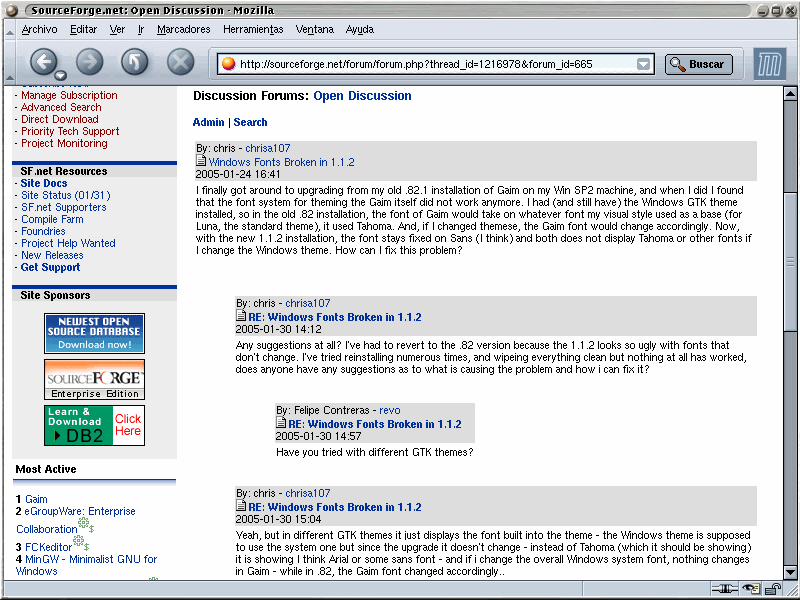
\includegraphics[bb=0 0 800 600, width=12cm, keepaspectratio]{img/foro1}
%    \caption{Página con enlaces a hilos}
%    \label{figura:foro_hilos}
% \end{figure}

%{\footnotesize
%\begin{verbatim}
%    From gaurav at gold-solutions.co.uk  Fri Jan 14 14:51:11 2005
%    From: gaurav at gold-solutions.co.uk (gaurav_gold)
%    Date: Fri Jan 14 19:25:51 2005
%    Subject: [Mailman-Users] mailman issues
%    Message-ID: <003c01c4fa40$1d99b4c0$94592252@gaurav7klgnyif>

%    Dear Sir/Madam,
%    How can people reply to the mailing list?  How do i turn off
%    this feature? How can i also enable a feature where if someone
%    replies the newsletter the email gets deleted?
%    Thanks

%    From msapiro at value.net  Fri Jan 14 19:48:51 2005
%    From: msapiro at value.net (Mark Sapiro)
%%    Date: Fri Jan 14 19:49:04 2005
 %   Subject: [Mailman-Users] mailman issues
%    In-Reply-To: <003c01c4fa40$1d99b4c0$94592252@gaurav7klgnyif>
%    Message-ID: <PC173020050114104851057801b04d55@msapiro>

%%    gaurav_gold wrote:
%    >How can people reply to the mailing list?  How do i turn off
%    this feature? How can i also enable a feature where if someone
%    replies the newsletter the email gets deleted?

%    See the FAQ
%    >Mailman FAQ: http://www.python.org/cgi-bin/faqw-mm.py
%    article 3.11
%\end{verbatim}
%}

\section{Objetivo Principal y Estructura}
\label{sec:objetivo}

%En esta sección se debería introducir la esctura de la memoria. Así:

%\begin{itemize}
%  \item En el primer capítulo se hace una intro al proyecto.

%  \item En el capítulo~\ref{chap:objetivos} (ojo, otra referencia automática) se muestran los objetivos del proyecto.

%  \item A continuación se presenta el estado del arte.

%  \item \ldots
%\end{itemize}

\section{Disponibilidad del Software}
\label{sec:objetivo}


%%%%%%%%%%%%%%%%%%%%%%%%%%%%%%%%%%%%%%%%%%%%%%%%%%%%%%%%%%%%%%%%%%%%%%%%%%%%%%%%
%%%%%%%%%%%%%%%%%%%%%%%%%%%%%%%%%%%%%%%%%%%%%%%%%%%%%%%%%%%%%%%%%%%%%%%%%%%%%%%%
% OBJETIVOS %
%%%%%%%%%%%%%%%%%%%%%%%%%%%%%%%%%%%%%%%%%%%%%%%%%%%%%%%%%%%%%%%%%%%%%%%%%%%%%%%%

\cleardoublepage % empezamos en página impar
\chapter{State of Art} % título del capítulo (se muestra)
\label{chap:state-of-art} % identificador del capítulo (no se muestra, es para poder referenciarlo)

\section{ElasticSearch} % título de sección (se muestra)
\label{sec:elasticsearch} % identificador de sección (no se muestra, es para poder referenciarla)

\textit{\textbf{Elasticsearch}} is an open-source, \textit{broadly-distributable}, \textit{readily-scalable}, \textit{enterprise-grade} search engine based on Lucene\footnote{\url{https://en.wikipedia.org/wiki/Apache\_Lucene}}. It provides a distributed, multitenant-capable full-text search engine with an HTTP web interface and schema-free JSON documents.

\subsection{History}
\label{subsec:elasticsearch-history}
\textit{Compass} was the predecessor to Elasticsearch and it was created by \textbf{Shay Banon} in 2004. Through the implementation of the third version of Compass, came the necessity of a \textit{"scalable search solution"}. This necessity would have meant a lot of work rewriting big pieces of code, so Shay decided to build \textit{"a solution built from the ground up to be distributed"} and used a common interface, \textit{JSON} over \textit{HTTP}, available for other programming languages, and not only \textit{Java}.

The first verision of Elasticsearch was released on February 2010.

\subsection{Basic Concepts}
\label{subsec:elasticsearch-basic-concepts}

All the following concepts definitions are extracted from the Elasticsearch documentation web page\footnote{\url{https://www.elastic.co/guide/en/elasticsearch/reference/current/_basic_concepts.html}}.

\begin{itemize}
    \item \textbf{Near Realtime (NRT)}:
        Elasticsearch is a near real time search platform.
        The practical meaning of this is that there is a little latency (about one second) from the moment you store a new document, to the moment it becomes available for searching.
    \item \textbf{Index}:
        An \textbf{index} is a set of documents that share some type of characteristics. For example, you can have an index for a shop product, another index for employee data and another for bill data. An index is identified by its name (in lowercase), and this name is used for several operations as: searching, deleting, updating, etc.
    \item \textbf{Shards \& Replicas}:
        The index data can reach a large size exceeding the available physical memory.
        But this problem can be fixed by defining multiple \textbf{shards}. Each shard is a portion of data from the index data. The number of shards is defined when the index is created.

        But there is still another potential problem. It always exists the possibility to have a failure on the network system and to loose a shard/node, so it is advisable to have \textbf{replicas} of our data. A replica is a copy of the index shards.
    \item \textbf{Type}:
        We can see a \textbf{type} like an object class, with fields of different data-types.

        In Elasticsearch a type is defined by its \textit{name} and its \textit{mappings}. The \textit{mappings} are a schema of the type, where it's defined the properties that our type has, and the data-type of each property, such as \textit{integer, string, etc.}.
    \item \textbf{Document}:
        As we said about \textit{types} being like classes, we could see a \textbf{document} like a record from a single class.
        Using the same example we used for \textit{indexes}, you can have a document for a single product, another document for a single employee and yet another for a single bill.
    \item \textbf{Node}:
        We can see a \textbf{node} like a single server, as a single unit that along with other nodes, make up a cluster. This node take part on cluster's indexing and searching tasks.
    \item \textbf{Cluster}:
        As we said in the previous definition, a \textbf{cluster} is made up with multiple nodes(servers). The cluster stores all the data and allows to search and index all this data across all nodes.
        A cluster is a collection of one or more nodes (servers) that together holds your entire data and provides federated indexing and search capabilities through all nodes.
\end{itemize}


\section{Kibana}
\label{sec:kibana}

\textbf{Kibana} is an \textit{Elasticsearch} open-source plug-in. It mainly works with Elasticsearch indexed data in order to represent it into different types of visualizations such as bar charts, scatter plot charts, pie charts, ...

Kibana, as an exploration tool, can be used to log and time series analytics, application monitoring, and operational intelligence use cases.

We can find another similar applications such as \textit{Grafna}\footnote{\url{https://grafana.com/}}, \textit{incubator-superset}\footnote{\url{https://github.com/apache/incubator-superset}} and \textit{Tableau}\footnote{\url{https://www.tableau.com/}}.

\subsection{Main Features}
\label{sec:kibana-functoinalities}

In the Figure~\ref{fig:kibana-nav-bar}, we can see the Kibana's \textit{nav-bar}. Now we are going to speak about a couple of features.
\begin{figure}
  \centering
  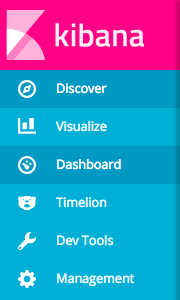
\includegraphics[height=6cm, keepaspectratio]{img/kibana-nav-bar}
  \caption{Kibana's nav-bar.}
  \label{fig:kibana-nav-bar}
\end{figure}

\begin{itemize}
    \item \textbf{Visualize}:

        \textit{Visualize} allows you to represent data with a specific type of chart. The represented data will be chosen from the available index on Elasticsearch. In addition to the Elasticsearch index, we have to choose which type of \textit{aggregations} are we going to use in order to extract our data. We can see an example on Figure~\ref{fig:kibana-visualization-example}.
        \begin{figure}
          \centering
          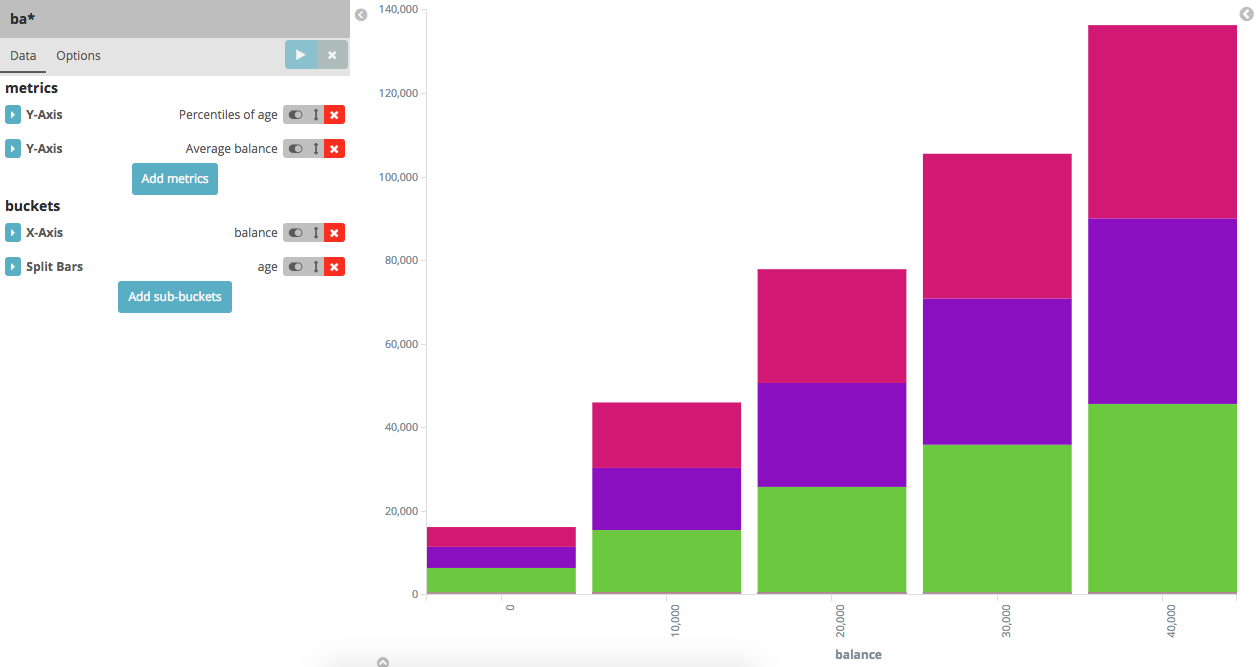
\includegraphics[width=15cm, keepaspectratio]{img/kibana-visualization-example}
          \caption{Visualization example.}
          \label{fig:kibana-visualization-example}
        \end{figure}
    \item \textbf{Dashboard}:

        The Kibana's dashboard functionality allows us to display a collection of saved visualizations and organize them by dragging and dropping. We can see an example on Figure~\ref{fig:kibana-dashboard-example}.
        \begin{figure}
          \centering
          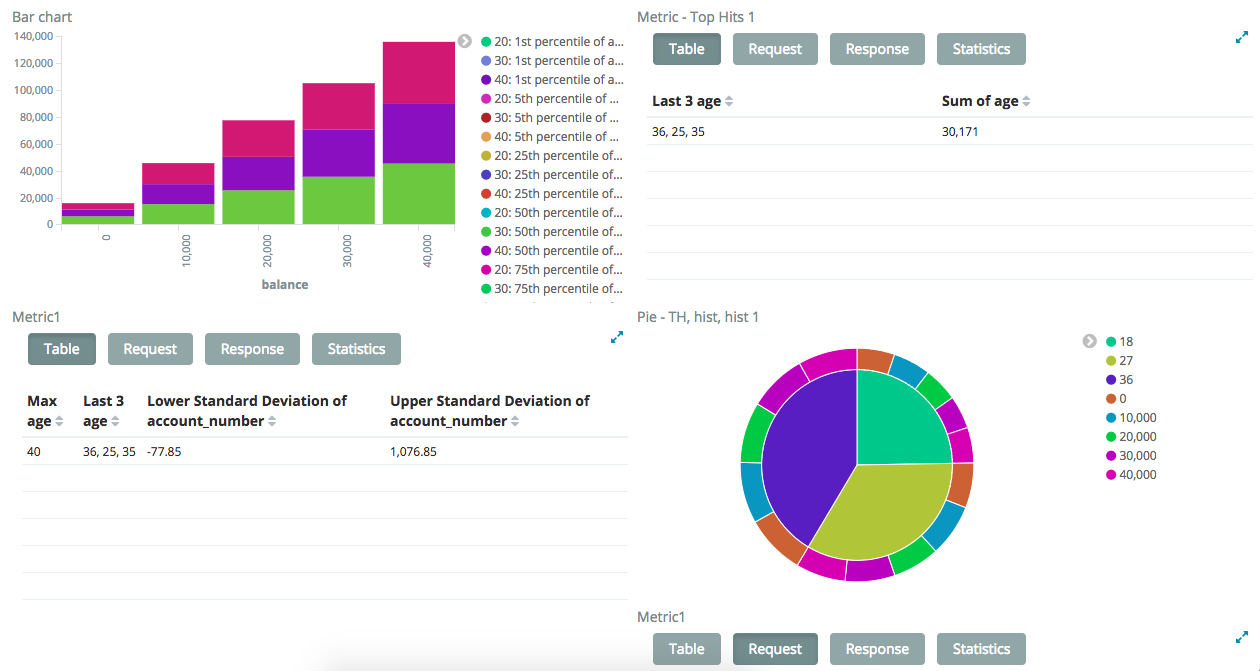
\includegraphics[width=15cm, keepaspectratio]{img/kibana-dashboard-example}
          \caption{Dashboard example.}
          \label{fig:kibana-dashboard-example}
        \end{figure}
\end{itemize}


\section{GitHub}
\label{sec:github}

"\textbf{GitHub} is a \textit{Web-based} \textbf{Git version control repository hosting service}". Github is used mainly for programming code. In addition to Git functionalities as \textit{deistributed version control} and \textit{source code management}, Github provides more features such as collaboration features for \textit{bug tracking} and for other porposes, task management, and \textit{wikis} for documentation porposes.

For the current project, a repository was created on \textit{Github} with the name of '\textit{Angular-ElasticSearch-Dashboard\_Interface}'\footnote{\url{https://github.com/islimane/Angular-ElasticSearch-Dashboard\_Interface}}.


\section{Webpack}
\label{sec:webpack}

"\textbf{Webpack} is an \textit{open-source JavaScript} module bundler". The main reason for using Webpack is to have a modular structure on your web application project. This allows you to have a cleaner code and make it more reusable and scalable. Webpack can be used from the command line or be configured with a config file named \textit{webpack.config.js}.


\section{Angular}
\label{sec:angular}

\textbf{Angular} is an open source \textit{web application platform} based on \textit{Typescript} and developed by Google and by a community of individuals and corporations.
Angular is commonly referred to as Angular 2.0 or later versions.

\subsection{Versions}
\label{sec:angular-versions}
Before Angular was created, there was a previous version called \textit{AngularJS} or Angular1.X. Angular was created as a complete rewrite of AngularJS.

\begin{itemize}
    \item 2.0.0:

        This was the first version of Angular. Its announcing was made at the \textit{ng-Europe} conference on September 2014. This version was build up from the ground and these were the main characteristics:
        \begin{itemize}
            \item Introduced the components hierarchy.
            \item Modules for core functionality, improving the speed of the Angular core.
            \item Possibility of using \textit{TypeScript} language. The use of this language is recommended by the Angular team.
            \item Improved \textit{dependency} injection.
            \item Dynamic loading.
            \item Reactive programming support using RxJS.
        \end{itemize}
        And much more features. The final version was released on September 14, 2016.
    \item 4.0.0:

        This version was called \textit{Angular 4} and was announced on 13 December 2016. Angular 3 was skipped due to some features already present on version 3.0.0 and to avoid confusion. This version introduced:
        \begin{itemize}
            \item \textit{Http} client.
            \item A new \textit{Rout Live Cycle}.
            \item Conditionally disable animations.
        \end{itemize}
    \item 5.0.0:

        This version was released on November 2017 and the main introduced features were:
        \begin{itemize}
            \item Support for progressive Web apps.
            \item A build optimizer and improvements related to \textit{Material Design}.
        \end{itemize}
\end{itemize}

\begin{figure}
  \centering
  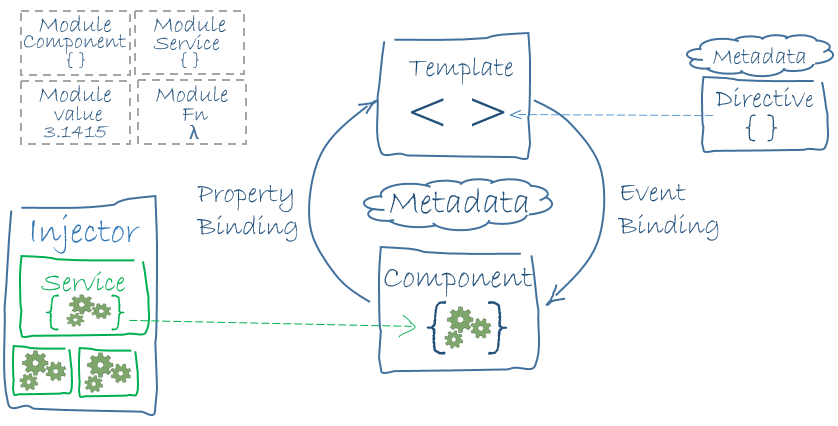
\includegraphics[width=13cm, keepaspectratio]{img/angular-architecture}
  \caption{Architecture of an Angular application}
  \label{fig:angular-architecture}
\end{figure}


\section{TypeScript}
\label{sec:typeScript}

"\textbf{TypeScript} is a free and open-source programming language developed and maintained by Microsoft. It is a strict syntactical \textit{superset} of \textit{JavaScript}, and adds optional static typing to the language".

\subsection{History}
\label{sec:typescript-history}

Before it was made public, \textit{TypeScript} gone through a two years of development process until it reached the 0.8 version. Then, was released on October 2012. Initially it had a lack of \textit{IDE} support, until 2013 when some IDE's began to have support for this language, such as \textit{Eclipse} with a dedicated pug-in, and some text editors such as \textit{Sublime}, \textit{Atom}, etc.

The reason TypeScript was created came from the necessity of a front-end programming language that fulfill the task of the development of complex and large-scale front-end applications, since JavaScript has shortcomings on that sense.

TypeScript is based on the \textit{EMACScript} approach, the reason why is because it is a standard and because it has support for \textit{class-based programming}.

\subsection{Language Features}
\label{sec:typescript-features}

\begin{itemize}
    \item Type annotations and compile-time type checking:

        TypeScript provides an optional static typing, with annotations, that is checked at compile time. If this typing it is not used, then the Javascript's dynamic typing is used. Here is an example:

        \begin{lstlisting}[language=javascript]
function planetMoons(planetName: string, moonsNum: number, spanish: boolean): any {
	if(spanish){
	    console.log('El planeta ' + planetName + ' tiene ' + moonsNum + ' lunas');
	}else{
	    console.log(planetName + '  planet has ' + moonsNum + ' moons');
	}

	return null;
}
        \end{lstlisting}
        \textit{string}, \textit{boolean} and \textit{number} are primitive types. For dynamic types it's used \textit{any}.

    \item Type inference.
    \item Type erasure.
    \item Interfaces.
    \item Enumerated type.
    \item Mixin.
    \item Generic.
    \item Namespaces.
    \item Tuple.
    \item Await.
    \item Classes (backported from EMACScript 2015).
    \item Modules (backported from EMACScript 2015).

\end{itemize}


\section{JavaScript}
\label{sec:typeScript}

"\textbf{JavaScript}, often abbreviated as JS, is a high-level, dynamic, weakly typed, prototype-based, multi-paradigm, and interpreted programming language. Alongside HTML and CSS, JavaScript is one of the three core technologies of World Wide Web content production". Generally, the main purpose of Javascript is to make pages interactive and develop online programs such as online games. Javascript is supported by most of the web browsers, for that reason, the majority of the websites employ it. There are multiple engines for Javascript, but all are standardized with the \textit{EMACScript} specification.

\subsection{History}
\label{sec:javascript-history}

Javascript came with the necessity of dynamism on web browsers. The founder of Netscape Communications, Marc Andreessen, thought that HTML needed a "glue language" to assemble component like images or plug-ins into the web markup. In 1995, Netscape Communications began to use \textit{Java} as a static programming language for Netscape Navigator, so the scripting language they had being searching for, had to be similar to Java and would complement it. Then, on May 1995, Brendan Eich wrote in 10 days this scripting language in order to compete against competing proposals. The first time this scripting language was called JavaScript was on December 1995, when the Netscape Navigator 2.0 beta 3 was released.

\subsection{Syntax}
\label{sec:javascript-syntax}

These are a few examples to illustrate the JavaScript syntax:

\begin{itemize}
    \item Variables:
        \begin{lstlisting}[language=javascript]
var x; // defines the variable x and assigns to it the special value "undefined" (not to be confused with an undefined value)
var y = 2; // defines the variable y and assigns to it the value 2
var z = "Hello, World!"; // defines the variable z and assigns to it a string entitled "Hello, World!"
        \end{lstlisting}
    \item Printing:
        \begin{lstlisting}[language=javascript]
console.log("Hello World!");
        \end{lstlisting}
    \item Functions:
        \begin{lstlisting}[language=javascript]
function add(a, b){
    return a + b;
}
add(1, 2); // returns 3
        \end{lstlisting}
\end{itemize}


\section{Lodash}
\label{sec:flexbox}

Lodash is a \textit{JavaScript} library that provides extra functions for tasks that are often required on data structure managing, a lot of them, not implemented on the main JavaScript functionality.

For example:
\begin{itemize}
    \item \textbf{\_.difference(array, [values])}: Creates an array of unique array values not included in the other provided arrays using SameValueZero for equality comparisons.
        \begin{lstlisting}[language=javascript]
_.difference([1, 2, 3], [4, 2]);
// returns [1, 3]
        \end{lstlisting}
    \item \textbf{\_.pluck(collection, path)}: Gets the property value of path from all elements in \textit{collection}.
        \begin{lstlisting}[language=javascript]
var users = [
  { 'user': 'barney', 'age': 36 },
  { 'user': 'fred',   'age': 40 }
];

_.pluck(users, 'user');
// returns ['barney', 'fred']
        \end{lstlisting}
\end{itemize}

As we can see, Lodash functions are called through the global variable "\_". All this functions can be found on the Lodash documentation\footnote{\url{https://lodash.com/docs/3.10.1}} page. This JavaScript library saves a lot of time when managing data structures.

There are other similar libraries such as \textit{UnderscoreJS}\footnote{\url{http://underscorejs.org/}}.


\section{jQuery}
\label{sec:jquery}

"\textit{jQuery} is a cross-platform JavaScript library designed to simplify the client-side scripting of HTML". jQuery it's the most used JavaScript library. jQuery's syntax is designed to make it easier to navigate a document, select DOM elements, create animations, handle events, and develop Ajax applications.

\subsection{History}
\label{sec:jquery-history}

    jQuery was originally released in January 2006 at BarCamp NYC by John Resig and was influenced by Dean Edwards' earlier cssQuery library. It is currently maintained by a team of developers led by Timmy Willison.

\subsection{Usage Examples}
\label{sec:jquery-examples}
\begin{itemize}
    \item HTML:
        \begin{lstlisting}[language=javascript]
<p>Hello</p>
        \end{lstlisting}
    \item JavaScript:
        \begin{lstlisting}[language=javascript]
$("p").clone().add( "<span>Again</span>" ).appendTo(document.body);
        \end{lstlisting}
    \item Result:

    See the result on Figure~\ref{fig:jquery-result-example}
        \begin{figure}
          \centering
          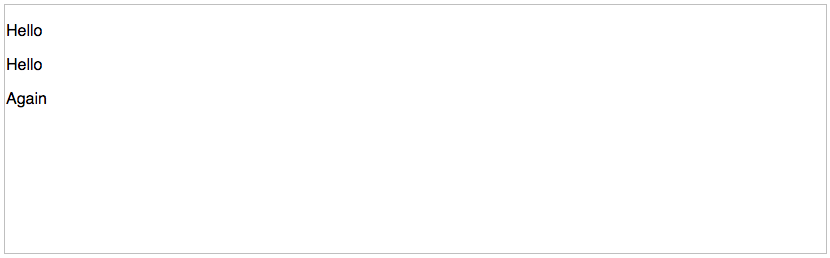
\includegraphics[width=13cm, keepaspectratio]{img/jquery-result-example}
          \caption{View result.}
          \label{fig:jquery-result-example}
        \end{figure}
\end{itemize}


\section{HTML5}
\label{sec:html5}

"\textbf{HTML5} is a markup language used for structuring and presenting content on the World Wide Web. It is the fifth and current major version of the HTML standard".

The \textit{World Wide Web Consortium} released HTML5 on October 2014, their goal was "to improve the language with support for the latest multimedia".

\subsection{Features}
\label{sec:html5-features}
These are some of the feature introduced in HTML5:
\begin{itemize}
    \item \textbf{Markup}:

        HTML5 introduces some elements that are commonly used on modern websites, they usually are replacements of old HTML elements, between these new elements we can find: \textit{<nav>}, \textit{<footer>}, \textit{<audio>}, \textit{<video>}, ...
    \item \textbf{New APIs}:

        HTML5 introduces \textit{application programming interfaces} or \textit{APIs} in addition to the markup elements that we have seen, such as \textit{Canvas}, \textit{Timed Media Playback}, \textit{Drag and Drop}, \textit{MIME type}, \textit{Web Messaging}, \textit{Web storage}, ... In this project we have mainly used \textit{Canvas} through the \textit{ChartJS} library.
\end{itemize}


\section{ChartJS}
\label{sec:chartjs}

\textbf{ChartJS} is a JavaScript library for producing dynamic, interactive data visualizations in web browsers, this is achieved by using the \textit{HTML5} \textit{canvas} element. With ChartJS you create different charts such as pie charts, bar charts, line charts, etc. You can find visual examples of each type on the ChartJS samples page\footnote{\url{http://www.chartjs.org/samples/latest/}}.

\subsection{Usage Examples}
\label{sec:chatjs-examples}

We have to instantiate the \textit{Chart} class in order to create a chart, an then assign it to a \textit{canvas} element on the DOM. The field \textit{type} indicates which chart are we going to use, and the field \textit{data} stores our chart info. Here is an example:

\begin{itemize}
    \item HTML:
        \begin{lstlisting}[language=javascript]
<canvas height='50' id='myChart' width='200'></canvas>
        \end{lstlisting}
    \item JavaScript:
        \begin{lstlisting}[language=javascript]
var ctx = document.getElementById("#myChart");
var myChart = new Chart(ctx, {
  type: 'bar',
  data: {
    labels: ["Red", "Blue", "Yellow"],
    datasets: [{
      label: '# of Votes',
      data: [12, 19, 3, 5, 2, 3],
      backgroundColor: [
        'rgba(255, 99, 132, 0.2)',
        'rgba(54, 162, 235, 0.2)',
        'rgba(255, 206, 86, 0.2)'
      ],
      borderColor: [
        'rgba(255,99,132,1)',
        'rgba(54, 162, 235, 1)',
        'rgba(255, 206, 86, 1)'
      ],
      borderWidth: 1
    }]
  }
});
        \end{lstlisting}
    \item Result:

    See the result on Figure~\ref{fig:chartjs-result-example}
    \begin{figure}
      \centering
      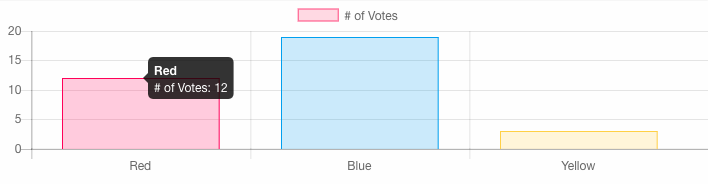
\includegraphics[width=13cm, keepaspectratio]{img/chartjs-result-example}
      \caption{View result.}
      \label{fig:chartjs-result-example}
    \end{figure}
\end{itemize}

There are a lot of libraries that allows you to render charts or graphs on a web page\footnote{\url{https://blog.sicara.com/compare-best-javascript-chart-libraries-2017-89fbe8cb112d}} such as \textit{C3.js}, \textit{Plotly.js}, etc. In this project we used ChartJS because it adapted well to the project requirements.


\section{SASS}
\label{sec:sass}

"\textbf{Sass} is a scripting language that is interpreted or compiled into \textit{Cascading Style Sheets} (CSS)". Sass uses two types of syntax. The first is original syntax, similar to \textit{Haml}\footnote{\url{https://en.wikipedia.org/wiki/Haml}}. The second is \textit{SCSS}, a syntaxt that uses blocks formatting like \textit{CSS}

\subsection{Features}
\label{sec:sass-features}
\begin{itemize}
    \item \textbf{Variables}:

        Sass allows defining variables using a dollar sign (\$).
        \begin{lstlisting}[language=javascript]
$primary-color: #3bbfce;

.content-navigation {
  border-color: $primary-color;
  color: darken($primary-color, 10%);
}
        \end{lstlisting}

    \item \textbf{Block Nesting}:

        Sass allows nesting different style blocks, this a improves the code structure, makes it more readable and saves lines of code.
        \begin{lstlisting}[language=javascript]
table.hl {
  margin: 2em 0;
  td.ln {
    text-align: right;
  }
}
        \end{lstlisting}

    \item \textbf{Loops}:

        With Sass you can create loops of style blocks, this feature helps to save code when you have similar \textit{id's} or \textit{classes}. Her is an example:
        \begin{lstlisting}[language=javascript]
$squareCount: 3
@for $i from 1 through $squareCount
  #square-#{$i}
   background-color: red
   width: 50px * $i
   height: 120px / $i
        \end{lstlisting}

    \item There are more Sass features such as \textit{arguments}, \textit{selector inheritance}, ... All of these features can be found on the Sass documentation web page\footnote{\url{http://sass-lang.com/documentation/file.SASS_REFERENCE.html}}.
\end{itemize}


\section{Flexbox}
\label{sec:flexbox}

"The \textit{CSS3 Flexible} Box, or \textbf{Flexbox}, is a layout mode intended to accommodate different screen sizes and different display devices". Flexbox is very useful when you have to organize your application view, so for example, sticking a \textit{footer} to the bottom of a page, designing a \textit{navigation bar}, creating a custom grid, ... is much easier using Flexbox.

Related to the Flexbox concept, it allows to manage an element width and the height to improve its fitting in the available space on the display regardless of the device that is being used. This elements are shrunken to prevent overflow or expanded to fill remaining space.

\subsection{Usage Examples}
\label{sec:chatjs-examples}

In order to use Flexbox styles, we have to apply the style "\textit{display: flex}" in our container element. Let's see a few Flexbox usage examples.

\begin{itemize}
    \item \textbf{flex-wrap}:

        Defines if flexbox items appear on a single line or on multiple lines within a flexbox container.
        \begin{lstlisting}[language=javascript]
flex-wrap: nowrap;
flex-wrap: wrap;
        \end{lstlisting}
        \begin{figure}
          \centering
          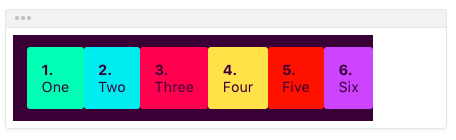
\includegraphics[width=11cm, keepaspectratio]{img/no-wrap-example}
          \caption{no-wrap example.}
          \label{fig:no-wrap-example}
        \end{figure}
        \begin{figure}
          \centering
          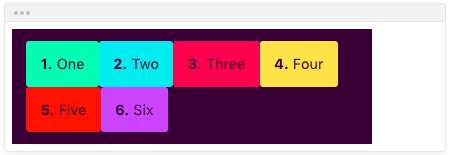
\includegraphics[width=11cm, keepaspectratio]{img/wrap-example}
          \caption{wrap example.}
          \label{fig:wrap-example}
        \end{figure}

    \item \textbf{justify-content}:

        Defines how flexbox items are aligned according to the main axis, within a flexbox container.
        \begin{lstlisting}[language=javascript]
justify-content: flex-end;
justify-content: center;
        \end{lstlisting}
        \begin{figure}
          \centering
          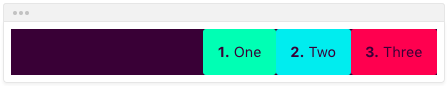
\includegraphics[width=11cm, keepaspectratio]{img/flex-end-example}
          \caption{flex-end example.}
          \label{fig:flex-end-example}
        \end{figure}
        \begin{figure}
          \centering
          
\includegraphics[width=11cm, keepaspectratio]{img/center-example}
          \caption{center example.}
          \label{fig:center-example}
        \end{figure}
\end{itemize}


%%%%%%%%%%%%%%%%%%%%%%%%%%%%%%%%%%%%%%%%%%%%%%%%%%%%%%%%%%%%%%%%%%%%%%%%%%%%%%%%
%%%%%%%%%%%%%%%%%%%%%%%%%%%%%%%%%%%%%%%%%%%%%%%%%%%%%%%%%%%%%%%%%%%%%%%%%%%%%%%%
% ESTADO DEL ARTE %
%%%%%%%%%%%%%%%%%%%%%%%%%%%%%%%%%%%%%%%%%%%%%%%%%%%%%%%%%%%%%%%%%%%%%%%%%%%%%%%%

%\cleardoublepage
%\chapter{Estado del arte}

%Descripción de las tecnologías que utilizas en tu trabajo.
%Con dos o tres párrafos por cada tecnología, vale.
%Se supone que aquí viene todo lo que no has hecho tú.

%Puedes citar libros, como el de Bonabeau et al. sobre procesos estigmérgicos~\cite{bonabeau:_swarm}. % Nota que el ~ añade un espacio en blanco, pero no deja que exista un salto de línea. Imprescindible ponerlo para las citas.

%También existe la posibilidad de poner notas al pie de página, por ejemplo, una para indicarte que visite la página de LibreSoft\footnote{\url{http://www.libresoft.es}}.

%\section{Sección 1}
%\label{sec:seccion1}

%Hemos hablado de cómo incluir figuras.
%Pero no hemos dicho nada de tablas.
%A mí me gustan las tablas.
%Mucho.
%Aquí un ejemplo de tabla, la Tabla~\ref{tabla:ejemplo}.

%\begin{table}
 %\begin{center}
%  \begin{tabular}{ | l | c | r |} % tenemos tres colummnas, la primera alineada a la izquierda (l), la segunda al centro (c) y la tercera a la derecha (r). El | indica que entre las columnas habrá una línea separadora.
%    \hline
%    1 & 2 & 3 \\ \hline % el hline nos da una línea vertical
%    4 & 5 & 6 \\ \hline
%    7 & 8 & 9 \\
%    \hline
%  \end{tabular}
%  \label{tabla:ejemplo}
%  \caption{Ejemplo de tabla}
% \end{center}
%\end{table}



%%%%%%%%%%%%%%%%%%%%%%%%%%%%%%%%%%%%%%%%%%%%%%%%%%%%%%%%%%%%%%%%%%%%%%%%%%%%%%%%
%%%%%%%%%%%%%%%%%%%%%%%%%%%%%%%%%%%%%%%%%%%%%%%%%%%%%%%%%%%%%%%%%%%%%%%%%%%%%%%%
% DISEÑO E IMPLEMENTACIÓN %
%%%%%%%%%%%%%%%%%%%%%%%%%%%%%%%%%%%%%%%%%%%%%%%%%%%%%%%%%%%%%%%%%%%%%%%%%%%%%%%%

\cleardoublepage
\chapter{Development}

\section{SCRUM Methodology}
\label{sec:scrum}

\textbf{SCRUM} is a work methodology designed mainly for \textit{software development}. The main philosophy of this methodology consists in subdividing the work into groups of smaller tasks, each group is called "\textit{Sprint}".

"Scrum is an iterative and incremental agile software development framework for managing product development".

A key principle of Scrum is the dual recognition:
\begin{itemize}
    \item Customers decision may change during the sprint development process (requirements volatility).
    \item There will be unpredictable challenges—for which a predictive or planned approach is not suited.
\end{itemize}

In the \textit{SCRUM} framework we can find three main roles:
\begin{itemize}
    \item \textbf{Product owner}: Ensures that the team delivers value to the business and represents both the product's stakeholders and the voice of the customer. The product owner manage the work process defining the product, adding stories to the backlog and prioritizing work.
    \item \textbf{Development team}: The team is the one that completes the tasks of a Sprint, building the product increments.
    \item \textbf{SCRUM master}: Removes the impediments, allowing the team to deliver product goals. The SCRUM master  filters all distracting influences from the development team.
\end{itemize}

On Figure~\ref{fig:scrum-framework} we can see a general SCRUM framework.
\begin{figure}
  \centering
  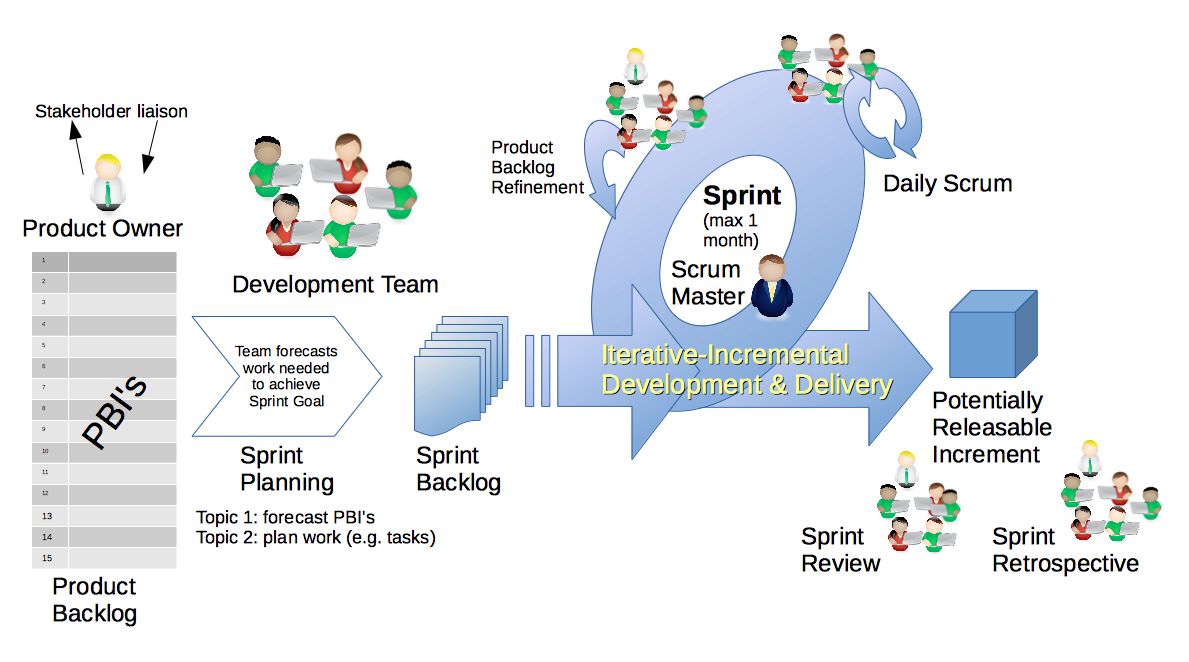
\includegraphics[width=14cm, keepaspectratio]{img/Scrum_Framework}
  \caption{SCRUM Framework}
  \label{fig:scrum-framework}
\end{figure}


\section{Sprint 1}
\label{sec:sprint-1}

\subsection{Key Objectives}
\label{sec:key-objectives}

The main goals or tasks for this sprint are:
\begin{itemize}
    \item Basic Elasticsearch interface which allows to visualize a simple metric. The data must come from Elastcsearch through an API request.
    \item Include more aggregations options and Index changing functionality.
\end{itemize}

\subsection{Implementing a simple metric request}
\label{sec:simple-request}
We are at the beginning of this project, the first thing we are going to do is to connect our Angular project to Elasticsearch. This can be achieved by installing the Elasticsearch library\footnote{\url{https://github.com/elastic/elasticsearch-js}} for Angular. This library will allow us to make requests to Elasticsearch through its javascript API.

We need an Elasticsearch client instance, this instance will give us the access to the Elasticsearch API. Elasticsearch, by default, it listens on the '9200' port, so we'll need to specify it too.
\begin{lstlisting}[language=javascript, caption=Client Insance, label=code:client-instance]
export class Elasticsearch {
	public clientElasticsearch: Client;
	constructor() {
		this.clientElasticsearch = new Client({
			host: 'localhost:9200',
			log: 'trace' // This is for debug purposes
		});
	}
...
}
\end{lstlisting}
This Elasticsearch class is created as an Angular \textbf{service}. In Angular, services are usually used for fetching data from the outside, this is what we are trying to achieve.

The next thing we are going to do is to request a simple "count" from Elasticsearch. In order to get this, we need to specify an Elasticsearch \textbf{index}.
\begin{lstlisting}[language=javascript]
...
public count(index): PromiseLike<number> {
	return this.clientElasticsearch.count({
			index: index
	}).then(
		response => response.count,
		this.handleError
	);
}
...
\end{lstlisting}
Now we just need to display the response.
\begin{lstlisting}[language=javascript]
// Html
<button (click)="displayData()">Display</button>
Count: <span>{{data}}</span>

// Typescript
...
data: number = 0;
...
displayData(): void {
	this.elasticsearch.count('bank')
	.then(count => this.data = count);
}
...
\end{lstlisting}


\subsection{Adding aggregations and dynamic index}
\label{sec:adding-aggregations}
First, in order to fetch the available indexes we are going to use the "cat" request, supported by the javascript API.
\begin{lstlisting}[language=javascript]
...
public getIndices(): PromiseLike<string[]>{
     return this.clientElasticsearch.cat.indices({
     	format: 'json'
     })
...
\end{lstlisting}
This method returns a JSON object, as we have specified in the "format" field. So we just need to parse this JSON response in order to build our indexes array. The next step is to retrieve all "number" fields for each index, since we are not going to implement aggregations that need another field type yet.
\begin{lstlisting}[language=javascript]
...
public getIndexNumFields(index): PromiseLike<string[]> {
 		return this.map(index).then(function(response){
...
\end{lstlisting}
The map method returns the index mappings, which we need to parse to build our "number fields" array.

The \textbf{PromiseLike} class is very useful because allows us to wait until the request is finished, in order to execute the appropriate callback function and manage the retrieved data asynchronously.

For now, we are going to include functionality for aggregations that works with fields of type "number" only. To achieve this we are going to use the "search" request provided by the Elasticsearch javascript API. This request returns a JSON object which we need to parse in a different way depending on the aggregation we are requesting, in order to get a displayable result.
\begin{lstlisting}[language=javascript]
...
// avg, sum, min, max, median, std_deviation, unique_count
public numFieldCalculation(index: string, aggs: any): PromiseLike<any>{
	return this.clientElasticsearch.search({
			"index": index,
			"body": {"size": 0, "aggs": aggs}
	})
...
\end{lstlisting}

The final stage view at the end of this sprint is shown on Figure~\ref{fig:sprint1-final-stage}.
\begin{figure}
  \centering
  \includegraphics[width=13cm, keepaspectratio]{img/final-stage-sprint1}
  \caption{Final stage view - Sprint 1}
  \label{fig:sprint1-final-stage}
\end{figure}

For a better understanding a general architecture for this sprint is shown on Figure~\ref{fig:sprint1-architecture}.
\begin{figure}
  \centering
  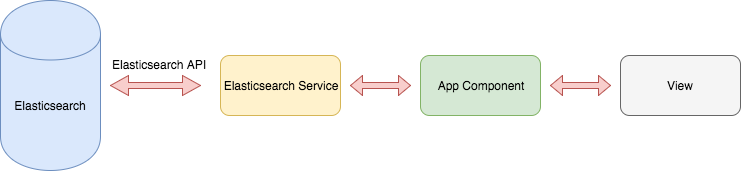
\includegraphics[width=13cm, keepaspectratio]{img/sprint1_architecture}
  \caption{Sprint 1 architecture.}
  \label{fig:sprint1-architecture}
\end{figure}


\section{Sprint 2}
\label{sec:sprint-2}
\subsection{Key Objectives}
\label{sec:key-objectives}

The main goals or tasks for this sprint are:
\begin{itemize}
    \item Finishing metrics functionality implementation.
    \item Implementing Data Table visualization functionality.
    \item Allow to load and save visualizations.
\end{itemize}

\subsection{Finishing metrics}
\label{sec:finishing-metrics}


\section{Sprint 3}
\label{sec:sprint-3}


\section{Sprint 4}
\label{sec:sprint-4}


\section{General Structure}
\label{sec:general-structure}

Si tu proyecto es un software, siempre es bueno poner la arquitectura (que es cómo se estructura tu programa a ``vista de pájaro'').

Por ejemplo, puedes verlo en la figura~\ref{fig:arquitectura}.

\begin{figure}
  \centering
  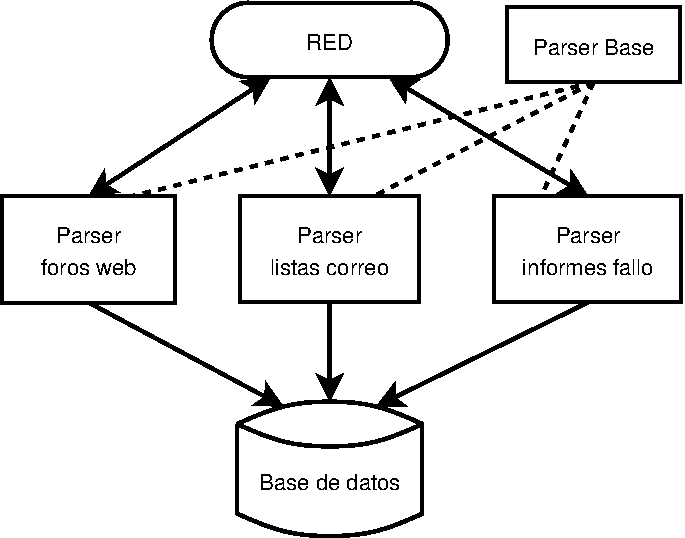
\includegraphics[width=9cm, keepaspectratio]{img/arquitectura}
  \caption{Estructura del parser básico}
  \label{fig:arquitectura}
\end{figure}

Si utilizas una base de datos, no te olvides de incluir también un diagrama de entidad-relación.


%%%%%%%%%%%%%%%%%%%%%%%%%%%%%%%%%%%%%%%%%%%%%%%%%%%%%%%%%%%%%%%%%%%%%%%%%%%%%%%%
%%%%%%%%%%%%%%%%%%%%%%%%%%%%%%%%%%%%%%%%%%%%%%%%%%%%%%%%%%%%%%%%%%%%%%%%%%%%%%%%
% RESULTADOS %
%%%%%%%%%%%%%%%%%%%%%%%%%%%%%%%%%%%%%%%%%%%%%%%%%%%%%%%%%%%%%%%%%%%%%%%%%%%%%%%%

\cleardoublepage
\chapter{Resultados}

En este capítulo se incluyen los resultados de tu trabajo fin de grado.

Si es una herramienta de análisis lo que has realizado, aquí puedes poner ejemplos de haberla utilizado para que se vea su utilidad.


%%%%%%%%%%%%%%%%%%%%%%%%%%%%%%%%%%%%%%%%%%%%%%%%%%%%%%%%%%%%%%%%%%%%%%%%%%%%%%%%
%%%%%%%%%%%%%%%%%%%%%%%%%%%%%%%%%%%%%%%%%%%%%%%%%%%%%%%%%%%%%%%%%%%%%%%%%%%%%%%%
% CONCLUSIONES %
%%%%%%%%%%%%%%%%%%%%%%%%%%%%%%%%%%%%%%%%%%%%%%%%%%%%%%%%%%%%%%%%%%%%%%%%%%%%%%%%

\cleardoublepage
\chapter{Conclusiones}
\label{chap:conclusiones}


\section{Consecución de objetivos}
\label{sec:consecucion-objetivos}

Esta sección es la sección espejo de las dos primeras del capítulo de objetivos, donde se planteaba el objetivo general y se elaboraban los específicos.

Es aquí donde hay que debatir qué se ha conseguido y qué no.
Cuando algo no se ha conseguido, se ha de justificar, en términos de qué problemas se han encontrado y qué medidas se han tomado para mitigar esos problemas.


\section{Aplicación de lo aprendido}
\label{sec:aplicacion}

Aquí viene lo que has aprendido durante el Grado/Máster y que has aplicado en el TFG/TFM. Una buena idea es poner las asignaturas más relacionadas y comentar en un párrafo los conocimientos y habilidades puestos en práctica.

\begin{enumerate}
  \item a
  \item b
\end{enumerate}


\section{Lecciones aprendidas}
\label{sec:lecciones_aprendidas}

Aquí viene lo que has aprendido en el Trabajo Fin de Grado/Máster.

\begin{enumerate}
  \item a
  \item b
\end{enumerate}


\section{Trabajos futuros}
\label{sec:trabajos_futuros}

Ningún software se termina, así que aquí vienen ideas y funcionalidades que estaría bien tener implementadas en el futuro.

Es un apartado que sirve para dar ideas de cara a futuros TFGs/TFMs.


%%%%%%%%%%%%%%%%%%%%%%%%%%%%%%%%%%%%%%%%%%%%%%%%%%%%%%%%%%%%%%%%%%%%%%%%%%%%%%%%
%%%%%%%%%%%%%%%%%%%%%%%%%%%%%%%%%%%%%%%%%%%%%%%%%%%%%%%%%%%%%%%%%%%%%%%%%%%%%%%%
% APÉNDICE(S) %
%%%%%%%%%%%%%%%%%%%%%%%%%%%%%%%%%%%%%%%%%%%%%%%%%%%%%%%%%%%%%%%%%%%%%%%%%%%%%%%%

\cleardoublepage
\appendix
\chapter{Manual de usuario}
\label{app:manual}


%%%%%%%%%%%%%%%%%%%%%%%%%%%%%%%%%%%%%%%%%%%%%%%%%%%%%%%%%%%%%%%%%%%%%%%%%%%%%%%%
%%%%%%%%%%%%%%%%%%%%%%%%%%%%%%%%%%%%%%%%%%%%%%%%%%%%%%%%%%%%%%%%%%%%%%%%%%%%%%%%
% BIBLIOGRAFIA %
%%%%%%%%%%%%%%%%%%%%%%%%%%%%%%%%%%%%%%%%%%%%%%%%%%%%%%%%%%%%%%%%%%%%%%%%%%%%%%%%

\cleardoublepage

% Las siguientes dos instrucciones es todo lo que necesitas
% para incluir las citas en la memoria
\bibliographystyle{abbrv}
\bibliography{memoria}  % memoria.bib es el nombre del fichero que contiene
% las referencias bibliográficas. Abre ese fichero y mira el formato que tiene,
% que se conoce como BibTeX. Hay muchos sitios que exportan referencias en
% formato BibTeX. Prueba a buscar en http://scholar.google.com por referencias
% y verás que lo puedes hacer de manera sencilla.
% Más información:
% http://texblog.org/2014/04/22/using-google-scholar-to-download-bibtex-citations/

\end{document}
